\section{Sistema distribuito}
\label{sec:sistema distribuito}
Come si accennava il precedenza, per lo sviluppo dell'applicazione è stato necessario ricorrere ad un sistema distribuito. Questo sistema, perno di tutta la trattazione, è invisibile all'utente ma di fondamentale importanza. Infatti, è colui che si occupa del processamento dei dati provenienti da Bitcoind, garantendo che nessun guasto infici sul risultato.
\\Il sistema elabora su più macchine distribuite per ottimizzare i tempi di risposta. In particolare, utilizza un "cluster Spark" (insieme di macchine) per ridistribuire il carico di lavoro equamente sui diversi nodi. Cosi facendo, ha la possibilità di elaborare grandi quantità di dati in real-time. Inoltre, utilizza la tecnica della replicazione dei dati così che, in caso di rottura di uno dei nodi, si possano recuperare le informazioni perse.
\\Terminata l'elaborazione dei dati, il cluster invia i risultati ai sistemi dediti al salvataggio e alla pubblicazione. Due, sono quelli dedicati alla storicizzazione permanente dei dati: Neo4j e Hadoop. Mentre per quanto riguarda la pubblicazione, i dati saranno inviati a Kafka (tramite un producer) che li renderà disponibili per essere fruiti. La scelta dei framework Hadoop e Kafka, è data dal fatto che sono entrambi capaci di lavorare in ambienti distribuiti. Diversa invece è la scelta di Neo4j, l'utilizzo di tale sistema, infatti, è dovuto al fatto che si adatta al meglio con l'idea di transazione, salvando i dati come grafi.

\begin{figure}[H]
	\centering
	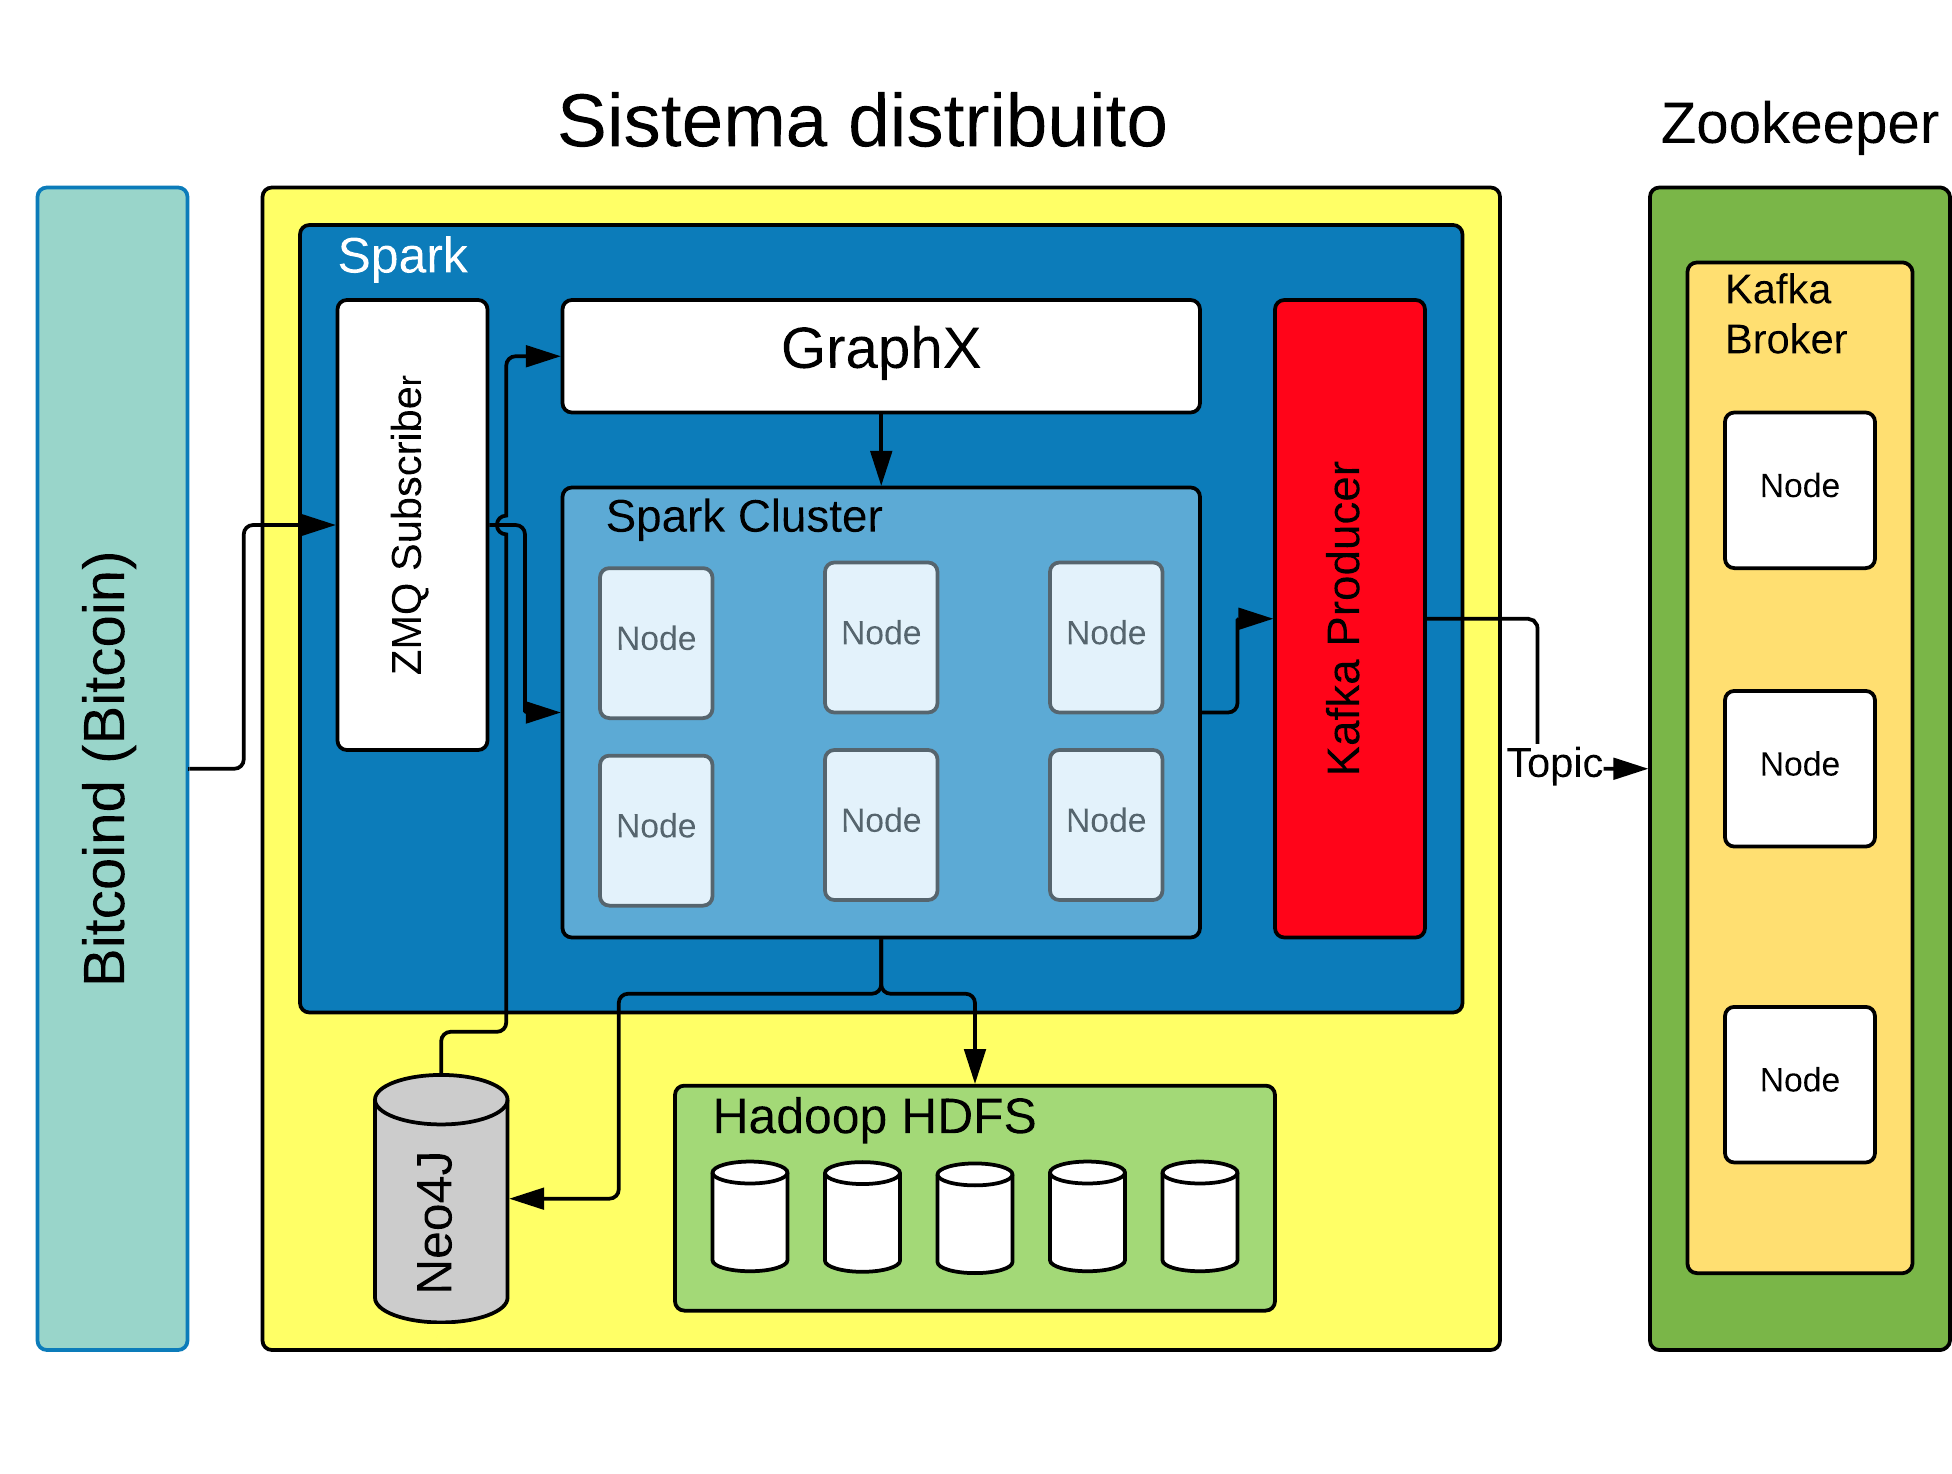
\includegraphics[width=\textwidth]{images/sistemaDistribuito.png}
	\caption{Architettura in dettaglio del sistema distribuito.}
	\label{fig:distribuitedSystemArchitetture}
\end{figure}